\chapter{Project Management}\label{ch:project_management}

This chapter outlines the project's management approach, including the development methodology, planning, and reflections on the process. It also considers legal and ethical issues and assesses key risks associated with the project.

\section{Methodology}
The project adopted an agile methodology, chosen for its flexibility, iterative development cycle, and emphasis on frequent customer feedback. The work involved incrementally building a series of interdependent features into vodle -- starting with a core delegation mechanism, and progressively expanding functionality to include ranked delegation, weighted delegation, and finally, per-option delegation. This iterative approach allowed each new feature to build directly upon the last, ensuring ongoing compatibility and adaptability in design decisions as the system evolved.

Agile methodology was particularly suitable for this project due to the involvement of an active ``customer'' figure: Jobst Heitzig, co-supervisor and original creator of vodle. Heitzig played a crucial role in defining system expectations and guiding design decisions based on practical, real-world considerations. Regular meetings, held fortnightly with both Jobst Heitzig and Markus Brill, facilitated continuous feedback and review of progress, enabling rapid adaptation of development plans. This feedback cycle closely reflects the Agile Manifesto's principles of early and continuous delivery, as well as close collaboration between developers and stakeholders \citep{agilemanifesto2001}.

Other project management approaches, such as Waterfall, were also evaluated but ultimately dismissed due to their inherent rigidity. Although Waterfall initially appeared attractive due to clearly defined phases and comprehensive documentation at each stage, its requirement to specify the complete project scope upfront was incompatible with the evolving nature of the project. Given the shorter time frame and the dynamic nature of feature requirements, the flexibility afforded by agile was critical to the project's success.

Scrum, one of the most widely adopted agile frameworks (used by approximately 63\% of agile teams \citep{versionone2020stateofagile}), was also considered. Its structured, sprint-based cycles, clear team roles, and structured ceremonies such as sprint planning and reviews were appealing for maintaining focused implementation and streamlined communication. However, the project's constraints -- limited availability due to academic commitments and a small team size -- made Scrum's daily stand-up meetings and fixed sprint lengths impractical. As a result, the project adopted an adapted agile approach: progress was reviewed every two weeks, effectively maintaining the advantages of frequent feedback without the constraints and scheduling pressures imposed by full Scrum ceremonies.

Each iteration of development produced a functional, testable feature that could be immediately evaluated and integrated into the broader system. This method significantly reduced the risk of late-stage integration issues and ensured steady, measurable progress throughout the project's duration. Overall, the agile methodology's iterative, feedback-oriented structure proved highly effective, meeting both the technical complexity and collaborative needs inherent in this work.
\section{Plan}

The project plan was organised into objectives (see Section \ref{ch:project_objectives}) that built on one another in sequence:

\begin{itemize}
    \item \textbf{Core Objective 1:} Implement a Core Delegation Model into Vodle.
    \item \textbf{Core Objective 2:} Implement Ranked Delegation into Vodle.
    \item \textbf{Core Objective 3:} Implement Weighted Delegation into Vodle.
    \item \textbf{Core Objective 4:} Implement Per-Option Delegation.
    \item \textbf{Extension Objective 1:} Simulate Delegation Mechanisms.
\end{itemize}

This objective-led structure was well-suited to the agile approach, allowing each milestone to be treated as an iteration with a deliverable at the end. A Gantt chart (see below) was created to visualise the project timeline and to track dependencies and progress.

\begin{figure}[H]
    \centering
    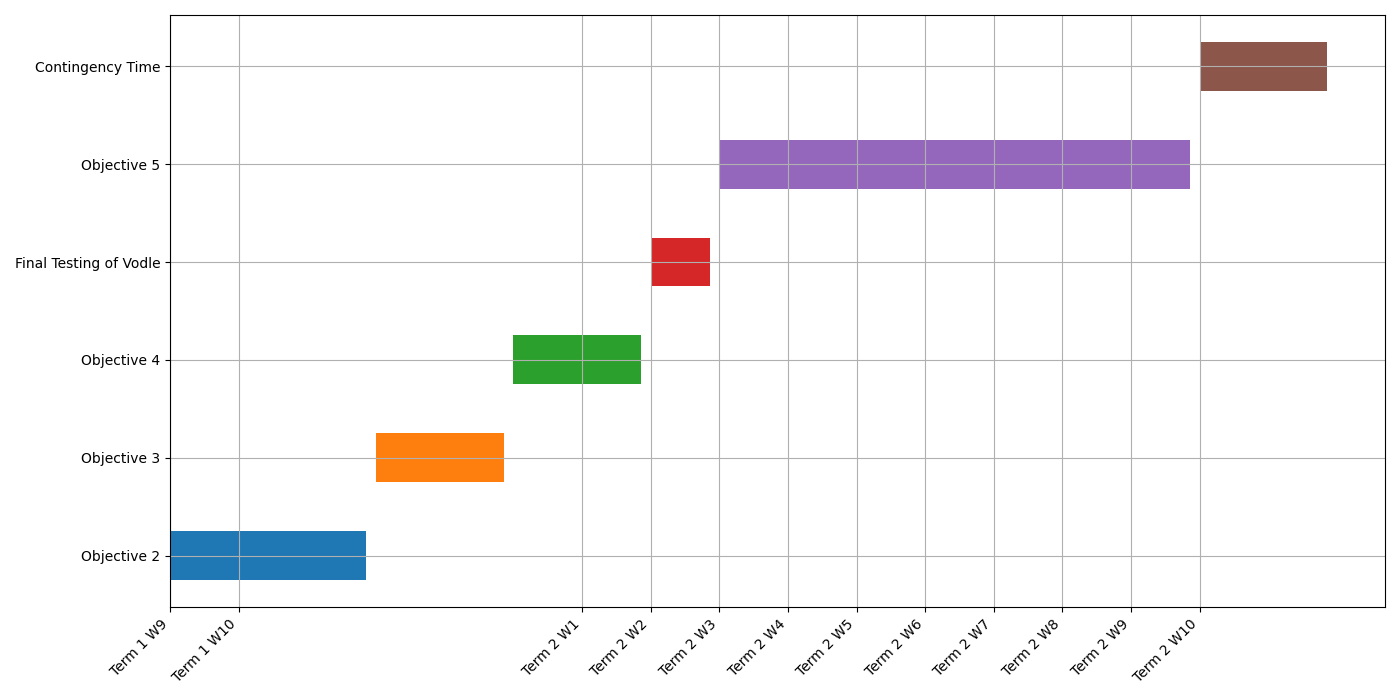
\includegraphics[width=0.8\textwidth]{../common/initial_gantt.png}
    \caption{Gantt chart illustrating the project plan from the progress report.}
    \label{fig:gantt}
\end{figure}


\section{Changes to the Project Plan}
The original project plan, illustrated in the Gantt chart (Figure~\ref{fig:gantt}), outlined a linear progression through the core objectives. However, several adjustments were made during the course of the project to reflect evolving priorities and unforeseen technical challenges.

The most significant change was the decision to de-scope the extension objective (simulating delegation mechanisms). This was prompted by two main factors. First, implementing the core objectives proved more technically demanding than initially anticipated -- particularly ranked delegation and weighted delegation. These challenges required more time and attention than expected, leaving limited capacity to complete the extension objective without compromising the quality of the core deliverables.

Second, during the background research phase, it became clear that similar investigations into delegation behaviour had already been conducted -- most notably by \citet{brill_liquid_2021}. Although their study did not use agent based modelling, instead using networks from synthetic and real-world networks (such as partial networks from Facebook, Twitter, Slashdot, etc.), it provided a comprehensive empirical evaluation of ranked delegation rules using various metrics such as maximum vote path length, average vote path rank, the number of isolated voters (voters without a delegation path) and many more.

Given the depth and relevance of these findings, replicating the analysis through agent-based modelling, especially within the project's limited timeframe, was deemed unnecessary. Instead, the project focused on fully delivering and refining the core objectives, which aligned more directly with vodle's platform goals and would have a better impact on the user experience of vodle.

A second change involved reversing the development order of objectives 3 and 4. Originally, objective 3 (weighted delegation) was scheduled to follow objective 2. However, during the Christmas development period, it became clear that objective 4 (per-option delegation) could be completed more quickly and required fewer algorithmic dependencies. To maintain development momentum, objective 4 was brought forward.

This adjustment helped mitigate project risk. Objective 4 involved minimal changes to the database schema and integrated easily with UI components developed for earlier objectives. In contrast, objective 3 introduced more complex computational logic and performance concerns, which demanded additional design, testing and changes to the database. Tackling objective 4 earlier helped avoid potential cascading delays and ensured a smoother integration process later in development.

\subsection{Actual Timeline vs Planned Timeline}
While the original project plan provided a clear sequence for implementing each objective, the actual progression deviated in several key areas due to technical challenges, interface considerations, and evolving priorities. Figure~\ref{fig:actual_gantt} (below) shows the actual timeline of the project, which can be compared to the original plan (Figure~\ref{fig:gantt}).
\begin{figure}[H]
    \centering
    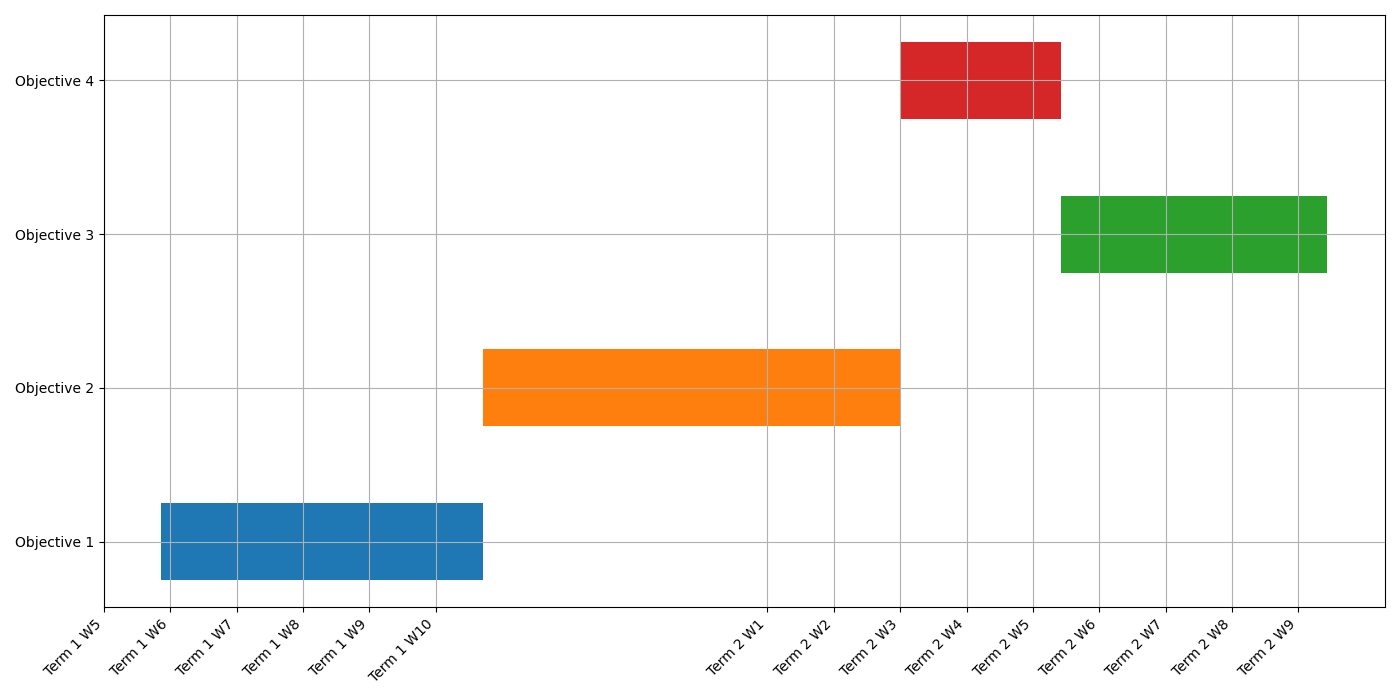
\includegraphics[width=0.8\textwidth]{../common/actual_gantt.png}
    \caption{Gantt chart illustrating the actual timeline of the project.}
    \label{fig:actual_gantt}
\end{figure}

The most significant deviations from the original plan included:

\begin{itemize}
    \item \textbf{Objective 1 (Core Delegation Model)} commenced approximately one week later than planned. This delay stemmed from the need for deeper familiarization with vodle's existing codebase, particularly its database schema and frontend architecture. Understanding these components was essential to ensure that new delegation features could integrate seamlessly without disrupting existing functionality. This initial exploration phase, while time consuming, was crucial for establishing a solid foundation for subsequent development.
    \item \textbf{Objective 2 (Ranked Delegation)} extended significantly beyond its initial timeframe. Originally scheduled for completion during the Christmas break, development continued until Term 2, Week 3. This extension was primarily due to the unforeseen complexities (as discussed in Section~\ref{sec:design_ranked_delegation}) which required both sophisticated transitive resolution logic and intuitive user interface feedback mechanisms, which proved more challenging than initially estimated.
    \item \textbf{Objectives 3 and 4}'s order was swapped, as discussed earlier in this section. While the original plan positioned Objective 3 (Weighted Delegation) to follow Objective 2, development logistics and dependency considerations prompted a shift to implement Objective 4 (Per-Option Delegation) first. This decision minimised integration risks, as Objective 4 required fewer schema modifications and built more directly on existing UI components, in particular those developed for Objective 2 (Ranked Delegation).
    \item \textbf{Extension Objective (Simulation)} was ultimately descoped from the project plan. This decision reflected both time constraints imposed by the extended development periods for core objectives and the discovery of existing comprehensive research on delegation behavior by \citet{brill_liquid_2021}. Focusing resources on delivering robust implementations of the core objectives was deemed more valuable than duplicating existing research.
\end{itemize}

Despite these deviations, the overall project structure remained intact and successful. The buffer period allocated at the end of Term 2 served its intended purpose as contingency time, effectively absorbing the delays in Objectives 1 and 2. This strategic planning ensured that despite timeline adjustments, the project remained on track for completion with all core objectives delivered to high quality standards.

The ability to adapt the project plan while maintaining focus on delivering the core functionality demonstrates the value of the chosen agile methodology. Rather than rigidly adhering to potentially unrealistic timelines, the flexible approach allowed for continuous reassessment and prioritisation based on evolving technical insights and stakeholder feedback.
\section{Risk Assessment}
The following section provides a detailed analysis of the risks identified in the risk assessment table below (see Table~\ref{tab:risk-assessment}). Each risk is discussed individually in detailed later on in the section, outlining its implications and the strategies proposed to mitigate potential issues.

\begin{table}[H]
\centering
\begin{tabular}{|p{4.5cm}|p{2cm}|p{8cm}|}
\hline
\textbf{Risk} & \textbf{Likelihood} & \textbf{Mitigation Strategy} \\
\hline
Breaking the live vodle site during development & Medium & Use Git branching to isolate development from production environments. Conduct local testing before deployment. \\
\hline
Feature complexity exceeds estimates & High & Prioritise core objectives and maintain flexibility in scope. \\
\hline
Lack of engagement from supervisors or stakeholders & Low & Maintain regular communication through scheduled meetings. \\
\hline
Data loss or corruption & Low & Use Git for version control and take regular local backups. \\
\hline
\end{tabular}
\caption{Key risks identified and their mitigation strategies}\label{tab:risk-assessment}
\end{table}

\subsection*{Breaking the Live Vodle Site During Development}

\textbf{Likelihood:} Medium

\textbf{Description:} Modifications to the existing vodle platform could unintentionally introduce downtime or impair existing functionality on the live website. Any disruptions could negatively impact real users' interactions, leading to dissatisfaction and loss of trust in the platform.

\textbf{Mitigation:} Development activities will utilise Git branching to isolate new code from the production environment. Features will be developed and rigorously tested in local or staging environments before integration with the live deployment. Incremental rollouts and thorough pre-deployment testing will further help identify potential problems early, allowing quick remediation or rollback.

\subsection*{Feature Complexity Exceeds Estimates}

\textbf{Likelihood:} High

\textbf{Description:} Advanced features such as ranked delegation and weighted delegaion may prove more complex than initially anticipated. Unexpected complexity can lead to delays, reduced functionality, or incomplete implementations, potentially affecting the project's timeline and deliverables.

\textbf{Mitigation:} Core objectives have been clearly defined and prioritised, ensuring focus remains on essential functionality. In cases of higher than anticipated complexity, resources will be redirected towards completing critical core features first, while the extension objective (agent based modelling) can be scaled back or postponed as needed. Regular agile reviews will monitor progress closely, facilitating early identification and management of complexity-related issues.

\subsection*{Lack of Engagement from Supervisors or Stakeholders}

\textbf{Likelihood:} Low

\textbf{Description:} Regular feedback and engagement from supervisors and stakeholders are crucial to ensure alignment with project goals, requirements, and user expectations. Insufficient feedback could result in misaligned implementations or objectives that do not fully meet user needs.

\textbf{Mitigation:} Fortnightly meetings have been scheduled with both the primary supervisor (Markus Brill) and the co-supervisor (Jobst Heitzig), who also fulfils the role of the project customer. This structured schedule ensures consistent opportunities for input and feedback. Additionally, a Telegram group chat is available to handle urgent queries and maintain ongoing dialogue.

\subsection*{Data Loss or Corruption -- Code}

\textbf{Likelihood:} Low

\textbf{Description:} Development activities pose a risk of code loss or corruption due to accidental deletion, unintended changes, or version conflicts. Such incidents could significantly delay development and necessitate additional time for recovery.

\textbf{Mitigation:} Version control will be rigorously maintained using Git, with frequent commits and descriptive commit messages ensuring traceability. Regular backups of the repository will be taken to safeguard against accidental loss, providing straightforward recovery paths when needed.

\subsection*{Data Loss or Corruption -- Database}

\textbf{Likelihood:} Low

\textbf{Description:} While unlikely, corruption of the CouchDB database during development could occur due to improper schema modifications or accidental changes.

\textbf{Mitigation:} No mitigation -- in the event of data corruption, the development database will be reset to its original state. As all data in the database is poll and user specific, it does not impact development as no important data is stored in the production environment.

\section{Risk Management Reflection}
This section evaluates how effectively the project's risk management strategies addressed both anticipated and unforeseen challenges. It examines which risks were realised, how mitigation strategies performed in practice, and identifies lessons learned that could inform future projects. 

\textbf{Breaking the Live Vodle Site During Development}

The use of Git branching strategies and comprehensive local testing successfully prevented any disruption to the live site. The separation between development and production environments ensured stability throughout the project lifecycle. This disciplined approach proved valuable despite adding some overhead to the development process.

\textbf{Feature Complexity Exceeds Estimates}

This materialised as the most significant risk, particularly during the implementation of ranked delegation (Objective 2) and weighted delegation (Objective 3). The algorithmic complexity and UI considerations extended development beyond initial estimates.
The strategy of prioritising core objectives proved invaluable, allowing the project to successfully deliver all essential functionality. The decision to descope the extension objective demonstrates effective risk management balancing ambition with practical constraints.
In hindsight, breaking complex features into smaller subtasks during planning might have improved estimation accuracy, though the agile methodology compensated through its inherent flexibility.

\textbf{Lack of Engagement from Supervisors or Stakeholders}

This risk did not take place. The fortnightly meetings and additional communication channels maintained strong engagement throughout the project. Jobst Heitzig's dual role as co-supervisor and customer representative provided crucial domain expertise and timely feedback on design decisions.

\textbf{Data Loss or Corruption}

No significant data loss incidents occurred. Git version control provided reliable tracking of code changes, while the lightweight approach to database management proved appropriate as no critical data was compromised.

\textbf{Summary}

Overall, the risk management approach proved effective in supporting project delivery despite several challenges. The most significant risk -- feature complexity exceeding estimates -- did occur and required timeline adjustments, but the contingency buffer and flexible scope management successfully mitigated its impact. The disciplined development approach prevented any disruption to the live site, while strong stakeholder engagement and version control systems effectively addressed the remaining identified risks. The experience highlighted the importance of integrating contingency time into project schedules and maintaining flexibility when dealing with technically complex features.

\section{Legal and Ethical Considerations}
As vodle may eventually be used to gather votes on sensitive topics, particular attention was paid to ensuring user privacy and system fairness throughout development.

Delegation chains are resolved internally within the browser and are never publicly exposed. A key design feature is that a delegation only becomes active when the invited user explicitly accepts the invitation. This ensures that no information about a user's voting intentions or delegation preferences is shared without their consent. The delegate only becomes aware of the relationship once they actively confirm it, and the delegator retains full control to revoke or modify the delegation at any time.

This mechanism protects the confidentiality of voter relationships and ensures that vote flows remain private unless both parties agree to the delegation. As such, even in a scenario where a vote is passed through multiple users, no individual along the chain gains access to the full path unless explicitly authorised.

Furthermore, no personal data was collected or processed for the purposes of this project. All stored information relates strictly to poll participation and delegation structures, with no link to identifiable personal attributes. As a result, no changes to vodle's terms of service were required, and the project remains compliant with relevant data protection and ethical standards.

\section{Overall/Self Reflection - TODO}
